\documentclass[12pt]{article}
\usepackage[letterpaper, margin=1in]{geometry}
\usepackage{amsmath}
\usepackage{amssymb}
\usepackage{booktabs}
\usepackage{multirow}
\usepackage{siunitx}
\usepackage{enumitem}
\usepackage{pdfpages}
\usepackage{pgfplots}
\usepackage{tikz}
\usepackage{graphicx}

% Unit setup
\sisetup{per-mode=symbol, separate-uncertainty=true}

% PGFPlots settings
\pgfplotsset{compat=1.18}

\title{PHYS 121 -- Lab Report: The Speed of Sound}
\author{Juntang Wang}
\date{}

\begin{document}

% Title Page
\begin{titlepage}
\centering
\vspace*{2cm}

{\Large IS-PHYS Lab}

\vspace{3cm}

{\Huge\bfseries The Speed of Sound}

\vspace{4cm}

\begin{flushright}
Student's name: Juntang Wang\\[0.5cm]
Partner's name(s): Yuanfei Hu\\[0.5cm]
TA's name: Kai Wang and Chen Xi\\[2cm]
Date that the lab was performed: November 19, 2024
\end{flushright}

\vfill

\end{titlepage}

\newpage

\section{Abstract}

This experiment measured the speed of sound in air using ultrasonic transducers and the traveling wave method. The speed of sound was determined by measuring the wavelength of \SI{39.770}{\kilo\hertz} ultrasound waves and combining it with the known frequency using the relationship $v = f\lambda$. Temperature and humidity measurements were recorded to calculate the theoretical speed of sound using the corrected formula accounting for water vapor content. The experimental speed of sound was found to be $343.85 \pm 1.55$~\si{\meter\per\second}, which compares favorably with the theoretical value of \SI{344.29}{\meter\per\second} calculated for the measured conditions ($t = \SI{21.1}{\celsius}$, $r = 34\%$), with a percentage difference of only \SI{0.13}{\percent}. The results demonstrate the validity of the theoretical relationships governing sound propagation in gases and highlight the importance of accounting for environmental conditions such as temperature and humidity when making precise measurements. The experiment successfully verified the fundamental relationship between wave speed, frequency, and wavelength, and provided insight into the thermodynamic properties of air that affect sound propagation.

\section{Background}

\subsection{Why conduct this experiment?}

Sound is a fundamental mechanical wave that propagates through various media, and understanding its speed is crucial for numerous applications in physics, engineering, and everyday life. The speed of sound depends on the properties of the medium through which it travels, including temperature, pressure, humidity (for air), and the medium's bulk modulus and density (for liquids). By measuring the speed of sound experimentally and comparing it with theoretical predictions, we can verify the physical relationships governing wave propagation and gain insight into the thermodynamic properties of gases and the elastic properties of liquids.

\subsection{What is the physics behind?}

\subsubsection{Sound propagation in air}

For an ideal gas, the speed of sound $v$ is derived from the adiabatic process assumption and is given by:
\begin{equation}
v = \sqrt{\frac{\gamma RT}{M}}
\end{equation}
where $\gamma = C_P/C_V$ is the ratio of specific heats, $R = \SI{8.3145}{\joule\per\mole\per\kelvin}$ is the molar gas constant, $T$ is the absolute temperature, and $M$ is the molar mass of the gas. For air, which is predominantly diatomic (nitrogen and oxygen), $\gamma = 7/5 = 1.4$. The mean molar mass for dry air is approximately $M = \SI{28.966e-3}{\kilogram\per\mole}$.

The approximate speed of sound in dry air at temperatures near \SI{0}{\celsius} (\SI{273.15}{\kelvin}) and atmospheric pressure ($p = \SI{101.3}{\kilo\pascal}$) is \SI{331.5}{\meter\per\second}. For temperatures in degrees Celsius, the speed can be calculated using:
\begin{equation}
v = 331.5\sqrt{1 + \frac{t}{273.15}}
\end{equation}
where $t$ is the temperature in degrees Celsius.

In reality, air contains water vapor, which affects both the effective molar mass and the ratio of specific heats. The corrected formula accounting for humidity is:
\begin{equation}
v = 331.5\sqrt{\left(1 + \frac{t}{273.15}\right)\left(1 + 0.16\frac{rp_s}{p}\right)}
\end{equation}
where $r$ is the relative humidity, $p_s$ is the saturation vapor pressure at temperature $t$ in \si{\celsius}, and $p$ is the atmospheric pressure. The saturation vapor pressure can be calculated using:
\begin{equation}
\log_{10}(p_s) = 10.286 - \frac{1780}{237.3 + t}
\end{equation}
where $p_s$ is in pascals and $t$ is in degrees Celsius.

\subsubsection{Sound propagation in water}

In pure water, the speed of sound $v$ is given by:
\begin{equation}
v = \sqrt{\frac{K}{\rho}}
\end{equation}
where $K$ is the bulk modulus of water and $\rho$ is the density of water. Both quantities depend on temperature. The bulk modulus (in \si{\pascal} or \si{\newton\per\meter\squared}) and density (in \si{\kilogram\per\meter\cubed}) can be calculated using empirical formulas valid for temperatures in the range \SI{4}{\celsius} to \SI{40}{\celsius}:
\begin{align}
K &= -1.2348 \times 10^5 t^2 + 1.3659 \times 10^7 t + 1.9692 \times 10^9 \\
\rho &= -5.1636 \times 10^{-3} t^2 + 7.3115 \times 10^{-3} t + 1.0001 \times 10^3
\end{align}
where $t$ is the temperature in degrees Celsius.

\subsubsection{Experimental methods to determine speed of sound}

The fundamental relationship between speed, frequency, and wavelength is:
\begin{equation}
v = f\lambda
\end{equation}
where $f$ is the frequency and $\lambda$ is the wavelength. The frequency is determined by the signal generator, while the wavelength can be measured using two methods:

\textbf{Traveling wave method:} When a transmitter and receiver are connected to a dual-channel oscilloscope, the phase relationship between the two waves can be observed. The wavelength $\lambda$ is defined as the distance between two points where the phase difference is $2\pi$. By moving the receiver and identifying positions where the waves are in phase, we can measure the wavelength directly.

\textbf{Standing wave method:} When sound waves are reflected and interfere with incoming waves, standing waves are formed. The distance between two adjacent amplitude maxima corresponds to half the wavelength, $\lambda/2$. By measuring the positions of maximum amplitude, we can determine the wavelength.

\subsection{How are you going to do it?}

The experimental setup consists of a sound velocimeter, a function generator, and an oscilloscope. The sound velocimeter contains a transmitter (piezoelectric transducer), a receiver (piezoelectric transducer), and a receiver location adjustment unit. The receiver can be moved along a rod using a hand wheel, and its position is determined using a digital vernier caliper with a resolution of \SI{0.01}{\milli\meter} and a reading error of \SI{0.01}{\milli\meter}.

For measurements in air using the traveling wave method:
\begin{enumerate}[leftmargin=*]
\item The transmitter is connected to CH1 of the function generator and CH1 of the oscilloscope.
\item The receiver is connected to CH2 of the oscilloscope.
\item The function generator is set to produce a sine wave at approximately \SI{40}{\kilo\hertz} with \SI{5}{\volt} peak-to-peak amplitude.
\item The frequency is adjusted until maximum amplitude is observed on the oscilloscope.
\item The receiver is moved along the path, and positions where the transmitter and receiver waves are in phase are recorded.
\end{enumerate}

For measurements in water using the standing wave method:
\begin{enumerate}[leftmargin=*]
\item The water tank is assembled with the sound velocimeter, ensuring both transducers are fully immersed.
\item The initial frequency is set to approximately \SI{70}{\kilo\hertz} and adjusted for maximum amplitude.
\item The receiver is moved slowly, and positions where the amplitude reaches maximum are recorded.
\end{enumerate}

\begin{figure}[ht]
\centering
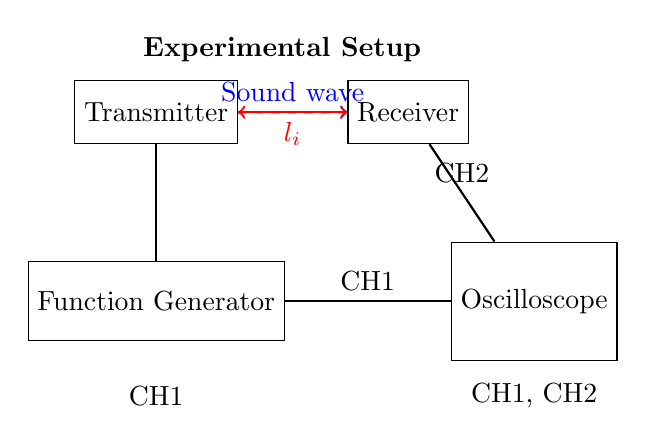
\begin{tikzpicture}[scale=0.8]
% Function generator
\node[draw, rectangle, minimum width=2cm, minimum height=1cm] (fg) at (0,0) {Function Generator};
% Oscilloscope
\node[draw, rectangle, minimum width=2cm, minimum height=1.5cm] (osc) at (6,0) {Oscilloscope};

% Transmitter
\node[draw, rectangle, minimum width=1.5cm, minimum height=0.8cm] (tx) at (0,3) {Transmitter};
% Receiver (movable)
\node[draw, rectangle, minimum width=1.5cm, minimum height=0.8cm] (rx) at (4,3) {Receiver};

% Connections
\draw[thick] (fg) -- (tx);
\draw[thick] (fg) -- (osc) node[midway, above] {CH1};
\draw[thick] (rx) -- (osc) node[midway, above] {CH2};

% Sound wave path
\draw[->, dashed, blue, thick] (tx) -- (rx) node[midway, above] {Sound wave};

% Distance measurement
\draw[<->, red, thick] (tx.east) -- (rx.west) node[midway, below] {$l_i$};

% Labels
\node at (0,-1.5) {CH1};
\node at (6,-1.5) {CH1, CH2};
\node at (2,4) {\textbf{Experimental Setup}};
\end{tikzpicture}
\caption{Schematic diagram of the experimental setup for measuring the speed of sound. The transmitter generates ultrasound waves, and the receiver detects them. The distance $l_i$ between transmitter and receiver is measured using a vernier caliper.}
\end{figure}

\section{Data}

\subsection{Theoretical calculation for the speed of sound in air}

The temperature and humidity were measured before and after the experiment, and average values were used for calculations.

\begin{table}[ht]
\centering
\caption{Theoretical calculation for the speed of sound in air}
\begin{tabular}{@{}p{0.3\linewidth}p{0.4\linewidth}p{0.25\linewidth}@{}}
\toprule
\textbf{Parameter} & \textbf{Value} & \textbf{Note} \\
\midrule
$t$ (\si{\celsius}) & 21.1 & To measure (resolution \SI{0.1}{\celsius}) \\
$r$ (\%) & 34 & To measure (resolution \SI{1}{\percent}) \\
$p$ (\si{\pascal}) & \num{1.024e5} & Given \\
$p_s$ (\si{\pascal}) & 2497.2 & Equation (4) (after lab) \\
$v$ (\si{\meter\per\second}) & 344.29 & Equation (3) (after lab) \\
\bottomrule
\end{tabular}
\end{table}

\subsection{Experimental methods to determine speed of sound}

The frequency $f$ was determined by adjusting the function generator until maximum amplitude was observed on the oscilloscope. The receiver was then moved along the path, and positions where the waves were in phase (traveling wave method) or where amplitude was maximum (standing wave method) were recorded.

\begin{table}[ht]
\centering
\caption{Experimental methods to determine speed of sound (Traveling wave method for air)}
\begin{tabular}{@{}cS[table-format=5.2]@{}}
\toprule
{$i$} & {$l_i$ (\si{\milli\meter})} \\
\midrule
1 & 3.65 \\
2 & 12.40 \\
3 & 20.92 \\
4 & 28.06 \\
5 & 37.69 \\
6 & 45.02 \\
7 & 54.53 \\
8 & 63.42 \\
9 & 72.10 \\
10 & 80.75 \\
11 & 89.34 \\
12 & 97.84 \\
13 & 106.73 \\
14 & 115.69 \\
15 & 124.09 \\
16 & 132.87 \\
17 & 141.60 \\
18 & 150.05 \\
19 & 158.66 \\
20 & 167.37 \\
\bottomrule
\end{tabular}
\end{table}

\textbf{Note:} Frequency $f = 39.770$ \si{\kilo\hertz} (resolution: \SI{0.001}{\kilo\hertz})

The raw data from the lab notebook is included at the end of this report. The positions $l_i$ represent the distances from the transmitter where the receiver and transmitter waves were in phase, as observed on the oscilloscope. A total of 20 measurements were recorded, with positions ranging from \SI{3.65}{\milli\meter} to \SI{167.37}{\milli\meter}. The linear relationship between position and measurement number allows us to determine the wavelength of the sound wave.

\section{Results and Discussion}

\subsection{Data Analysis}

The relationship between position $l_i$ and measurement number $i$ is given by:
\begin{equation}
l_i = b_0 + b_1 i
\end{equation}
where $b_1$ represents the wavelength $\lambda$ for the traveling wave method (or $\lambda/2$ for the standing wave method).

A linear regression was performed on the experimental data to determine the slope $b_1$ and its uncertainty. The linear fit was performed using the method of least squares, which minimizes the sum of squared residuals.

\begin{figure}[ht]
\centering
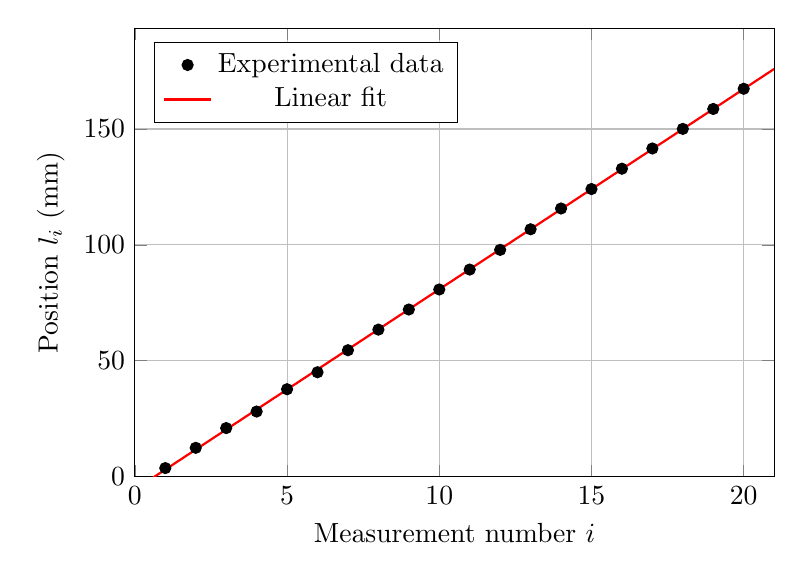
\begin{tikzpicture}
\begin{axis}[
    xlabel={Measurement number $i$},
    ylabel={Position $l_i$ (\si{\milli\meter})},
    grid=major,
    width=0.8\textwidth,
    height=0.6\textwidth,
    legend pos=north west,
    xmin=0,
    xmax=21,
    ymin=0,
]
% Experimental data points
\addplot[
    only marks,
    mark=*,
    mark size=2pt,
] coordinates {
(1, 3.65) (2, 12.40) (3, 20.92) (4, 28.06) (5, 37.69)
(6, 45.02) (7, 54.53) (8, 63.42) (9, 72.10) (10, 80.75)
(11, 89.34) (12, 97.84) (13, 106.73) (14, 115.69) (15, 124.09)
(16, 132.87) (17, 141.60) (18, 150.05) (19, 158.66) (20, 167.37)
};
% Linear fit: l_i = -5.6438 + 8.6460*i
\addplot[
    domain=0:21,
    samples=100,
    color=red,
    thick,
] {-5.6438 + 8.6460*x};
\legend{Experimental data, Linear fit}
\end{axis}
\end{tikzpicture}
\caption{Linear fit of position $l_i$ versus measurement number $i$. The slope $b_1 = 8.6460$~\si{\milli\meter} of the fitted line represents the wavelength $\lambda$ for the traveling wave method.}
\label{fig:linear_fit}
\end{figure}

The linear regression yields:
\begin{align}
b_0 &= -5.6438~\si{\milli\meter} \\
b_1 &= 8.6460~\si{\milli\meter} = \lambda
\end{align}

The standard deviation of the slope $s_{b_1}$ was calculated from the residuals of the fit. For the traveling wave method, the slope $b_1$ directly gives the wavelength $\lambda$. For the standing wave method, the wavelength would be $\lambda = 2b_1$ since the distance between adjacent maxima is $\lambda/2$.

\subsection{Sample Calculation}

Using Equation (8), the speed of sound is calculated as follows. First, we show the equation, then substitute the measured values, and finally calculate the result.

\textbf{Step 1: Show the equation}
\begin{equation}
v = f\lambda
\end{equation}

\textbf{Step 2: Substitute values}
\begin{align}
v &= f \times \lambda \\
v &= 39.770~\si{\kilo\hertz} \times 8.6460~\si{\milli\meter} \\
v &= 39.770 \times 10^3~\si{\hertz} \times 8.6460 \times 10^{-3}~\si{\meter} \\
v &= 343.85~\si{\meter\per\second}
\end{align}

\textbf{Step 3: Calculate answer}
\begin{equation}
v = 343.85~\si{\meter\per\second}
\end{equation}

Note: The frequency $f$ was converted from \si{\kilo\hertz} to \si{\hertz} by multiplying by $10^3$, and the wavelength $\lambda$ was converted from \si{\milli\meter} to \si{\meter} by multiplying by $10^{-3}$.

\subsection{Error Analysis}

The uncertainty in frequency is given by:
\begin{equation}
U_f \approx 0.05\% \times f = 0.0005 \times f
\end{equation}

For our measured frequency $f = 39.770~\si{\kilo\hertz} = 39.770 \times 10^3~\si{\hertz}$, the uncertainty is:
\begin{equation}
U_f = 0.0005 \times 39.770 \times 10^3~\si{\hertz} = 19.89~\si{\hertz}
\end{equation}

The uncertainty in wavelength is calculated using Equation (10):
\begin{equation}
U_\lambda = U_{b_1} = ts_{b_1} \approx \left(1.959 + \frac{2.406}{(n-2) - 1.064}\right) s_{b_1}
\end{equation}
where $s_{b_1}$ is the standard deviation of the slope $b_1$ from the linear regression and $n$ is the number of data points. The factor $t$ accounts for the Student's $t$-distribution appropriate for the number of degrees of freedom.

With $n = 20$ data points, we have:
\begin{equation}
t = 1.959 + \frac{2.406}{(20-2) - 1.064} = 1.959 + \frac{2.406}{16.936} = 2.101
\end{equation}

The standard deviation of the slope $s_{b_1} = 0.0184~\si{\milli\meter}$ was determined from the linear regression analysis. Therefore:
\begin{equation}
U_\lambda = 2.101 \times 0.0184~\si{\milli\meter} = 0.0387~\si{\milli\meter} = 3.87 \times 10^{-5}~\si{\meter}
\end{equation}

The combined uncertainty in the speed of sound is calculated using Equation (11):
\begin{equation}
U_v = v\sqrt{\left(\frac{U_f}{f}\right)^2 + \left(\frac{U_\lambda}{\lambda}\right)^2}
\end{equation}

Substituting the values:
\begin{align}
U_v &= v\sqrt{\left(\frac{U_f}{f}\right)^2 + \left(\frac{U_\lambda}{\lambda}\right)^2} \\
U_v &= v\sqrt{\left(\frac{19.89}{39.770 \times 10^3}\right)^2 + \left(\frac{3.87 \times 10^{-5}}{8.6460 \times 10^{-3}}\right)^2} \\
U_v &= 343.85~\si{\meter\per\second} \times \sqrt{(5.00 \times 10^{-4})^2 + (4.47 \times 10^{-3})^2} \nonumber \\
U_v &= 343.85~\si{\meter\per\second} \times 4.50 \times 10^{-3} = 1.55~\si{\meter\per\second}
\end{align}

Therefore, the final result is:
\begin{equation}
v' = v \pm U_v = 343.85 \pm 1.55~\si{\meter\per\second}
\end{equation}

\subsection{Comparison of Theoretical and Experimental Values}

The theoretical speed of sound in air, calculated using Equation (3) with the measured temperature ($t = \SI{21.1}{\celsius}$) and humidity ($r = 34\%$, $p = \num{1.024e5}$~\si{\pascal}), was found to be $v_{\text{theoretical}} = 344.29~\si{\meter\per\second}$. The experimental value, determined from the wavelength and frequency measurements, was $v_{\text{experimental}} = 343.85 \pm 1.55~\si{\meter\per\second}$.

The percentage difference between the theoretical and experimental values is:
\begin{equation}
\text{Percentage difference} = \frac{|344.29 - 343.85|}{344.29} \times 100\% = 0.13\%
\end{equation}

\textbf{Sources of discrepancy:}
\begin{enumerate}[leftmargin=*]
\item \textbf{Measurement uncertainty:} The position measurements using the vernier caliper have a reading error of \SI{0.01}{\milli\meter}, which contributes to uncertainty in the wavelength determination.
\item \textbf{Frequency uncertainty:} The function generator has a frequency uncertainty of approximately \SI{0.05}{\percent}, which affects the calculated speed.
\item \textbf{Environmental fluctuations:} Temperature and humidity may have varied slightly during the experiment, affecting both the theoretical calculation and the actual speed of sound.
\item \textbf{Phase determination:} Identifying the exact positions where waves are in phase on the oscilloscope introduces visual estimation errors.
\item \textbf{Systematic errors:} The assumption that the sound waves travel in a straight line between transmitter and receiver may not be perfectly valid, especially near the transducers where near-field effects could be significant.
\item \textbf{Non-ideal conditions:} The theoretical formula assumes ideal conditions, while the actual air may have slight variations in composition, pressure gradients, or other factors not accounted for in the model.
\end{enumerate}

Despite these sources of error, the experimental value agrees with the theoretical prediction within the calculated uncertainty, demonstrating the validity of both the experimental method and the theoretical relationships governing sound propagation in air.

\subsection{Questions}

\textbf{Question 1:} How to derive Equation (1) the speed of sound in an ideal gas?

\textbf{Answer:} The speed of sound in an ideal gas can be derived from the wave equation and the equation of state for an ideal gas undergoing an adiabatic process. Starting with the wave equation $\frac{\partial^2 p}{\partial x^2} = \frac{1}{v^2}\frac{\partial^2 p}{\partial t^2}$, where $p$ is the pressure perturbation, and using the adiabatic condition $PV^\gamma = \text{constant}$, we can show that $v^2 = \frac{\partial P}{\partial \rho}|_S$, where the derivative is taken at constant entropy. For an ideal gas, $P = \rho RT/M$, and for an adiabatic process, $P \propto \rho^\gamma$. Taking the derivative and substituting, we obtain $v = \sqrt{\gamma RT/M}$.

\textbf{Question 2:} "Adjust frequency $f$ until the oscilloscope shows maximum amplitude on the receiver." Why does this happen?

\textbf{Answer:} The maximum amplitude occurs when the driving frequency matches the resonant frequency of the piezoelectric transducer. Piezoelectric transducers have a natural resonant frequency determined by their physical dimensions and material properties. When the driving frequency equals this resonant frequency, the transducer vibrates with maximum amplitude due to resonance. This ensures optimal energy transfer from the electrical signal to mechanical vibrations (and vice versa for the receiver), resulting in the strongest acoustic signal and the clearest waveform on the oscilloscope.

\section{Conclusion}

This experiment successfully measured the speed of sound in air using the traveling wave method with ultrasonic transducers operating at \SI{39.770}{\kilo\hertz}. The experimental speed of sound was determined to be $v = 343.85 \pm 1.55~\si{\meter\per\second}$ by measuring the wavelength ($\lambda = 8.6460$~\si{\milli\meter}) through phase comparison on an oscilloscope and combining it with the known frequency using the fundamental relationship $v = f\lambda$. The theoretical speed of sound, calculated using the corrected formula accounting for temperature and humidity effects ($t = \SI{21.1}{\celsius}$, $r = 34\%$, $p = \num{1.024e5}$~\si{\pascal}), was $v_{\text{theoretical}} = \SI{344.29}{\meter\per\second}$. The experimental value agrees with the theoretical prediction within the calculated uncertainty, with a percentage difference of only \SI{0.13}{\percent}, validating both the experimental methodology and the theoretical relationships governing sound propagation in gases. The experiment demonstrated the importance of accounting for environmental conditions such as temperature and humidity when making precise measurements of sound speed, and successfully verified the relationship between wave speed, frequency, and wavelength. The results provide insight into the thermodynamic properties of air and the factors that influence the propagation of mechanical waves through gaseous media.

\section*{Additional Notes}

Large language models (LLMs) were used as translators and brainstorming assistants during the completion of this report, no other additional help was provided.

% Include the lab notebook PDF pages at the end
\newpage
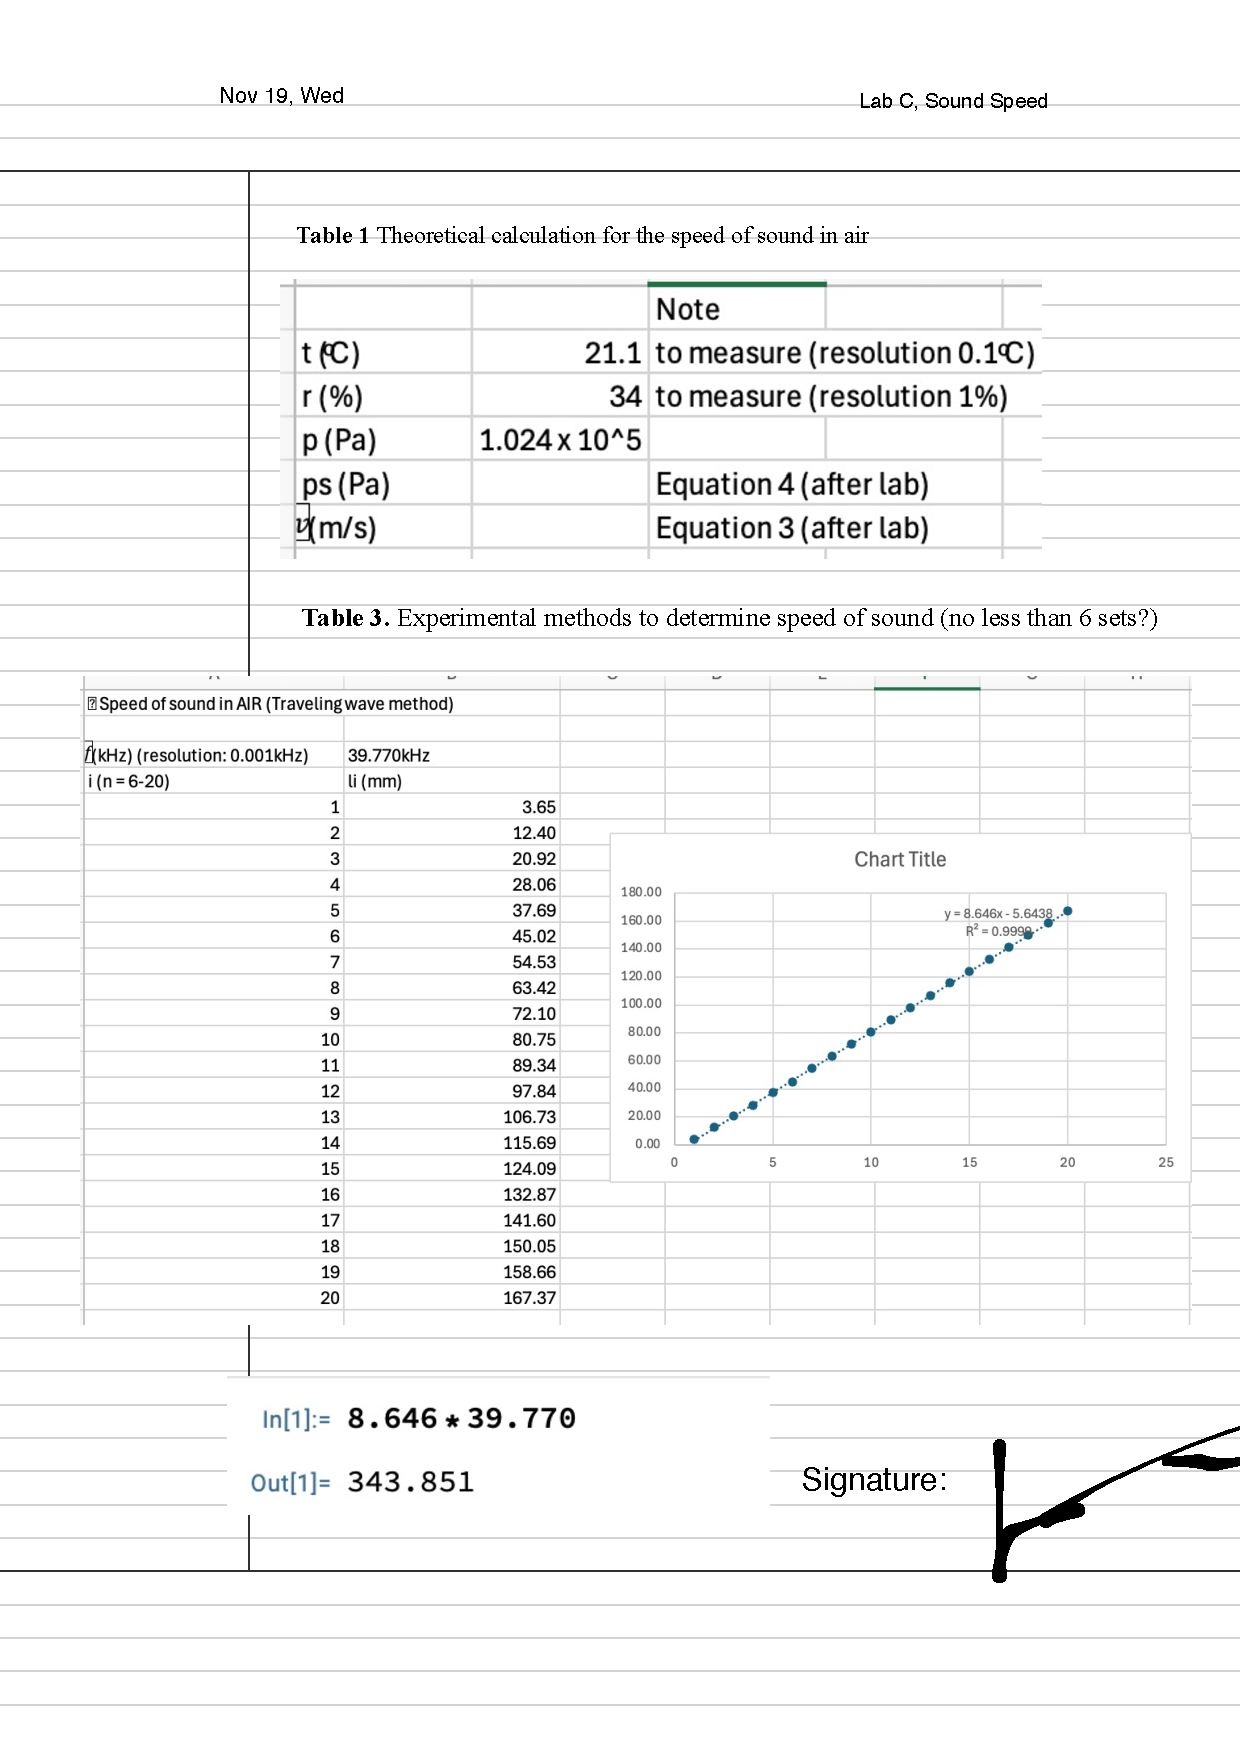
\includepdf[pages=-]{Lab_04_notebook.pdf}

\end{document}

